\documentclass[11pt]{article}            

\usepackage{graphicx}
\usepackage{listings}
\usepackage{amssymb}
\usepackage{epstopdf}
\usepackage{hyperref}
\DeclareGraphicsRule{.tif}{png}{.png}{`convert #1 `dirname #1`/`basename #1 .tif`.png}

\usepackage[T1]{fontenc}
\usepackage[utf8x]{inputenc}

\newcommand\fnurl[2]{%
  \href{#2}{#1}\footnote{\url{#2}}%
}

\title{Srovnání implementací Key Word in Context}
\author{Václav Purchart, Alena Varkočková}
\date{\today}                                         

\begin{document}
\maketitle

KWIC je zkráceně Key Word in Context. Jedná se o indexovací systém, který na vstupu přijímá seřazenou množinu řádků, přičemž každý řádek je složený ze seřazené množiny slov. Na každé řádce je pak proveden “circular shift” čili opakované hození slov tak, že je vždy první slovo odejmuto a vloženo na konec a každý takovýto posun vytváří novou řádku. Výstupem je abecedně seřazená množina těchto řádků.

KWIC byl naimplementován pomocí čtyřech různých architektonických stylů - Shared Memory, Abstract Data Types, Event Based - Implicit invocation a Pipe-and-Filter. U všech bylo zároveň naimplementováno vyhledávání a první tři zmíněné používají pro Circular Shifter, Alphabetizer a Output ukládání ve fomě indexů + offsetů.

\section{Shared memory}

Program je dekomponován do pěti modulů - input, shifter, alphabetizer, output a search. Všechny tyto jsou řízeny třídou Main, která je zodpovědná za jejich volání. Jednotlivé moduly data sdílí ve sdíleném uložišti, kam mají všichni read-write přístup. Ke konfliktům ale nedochází vzhledem k tomu, že třída Main zajišťuje sekvenční přístup k datům.

\begin{figure}[htbp]
	\caption{Shared memory - class diagram}
		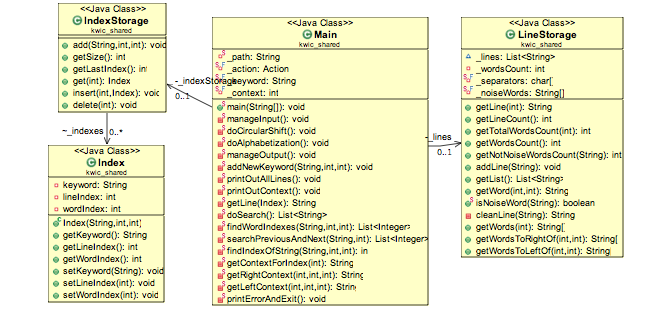
\includegraphics[width=13cm]{shared}
	\label{fig:shared}
\end{figure}

\section{Abstract data types}

Stejně jako Shared memory, také toto řešení vzniklo dekompozicí do pěti modulů. Hlavní změnou ale je, že data již nejsou nadále sdílena v jednom uložišti. Místo toho je k datům zajištěn přístup přes public metody třídy daného modulu. 

\begin{figure}[htbp]
	\caption{Abstract data types - class diagram}
		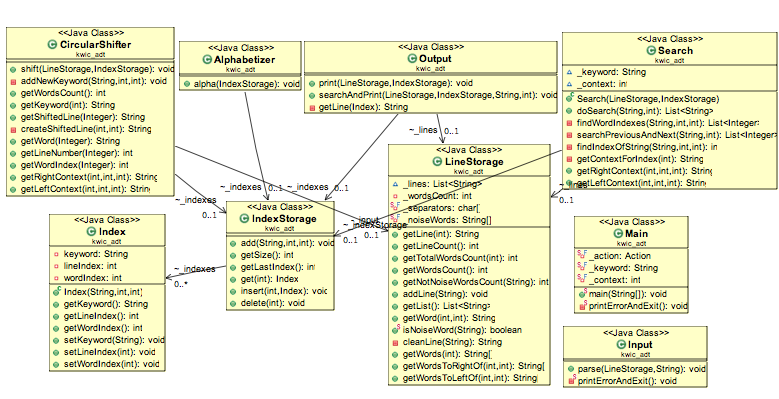
\includegraphics[width=13cm]{adt}
	\label{fig:adt}
\end{figure}

\section{Event based - implicit invocation}

Hlavní změnou této implementace KWIC je způsob zpracování. Jednotlivé moduly se registrují jako Observery reagující na změnu v LineStorage. CircularShifter je tedy volán po každém přidání nové řádky. Poté co na řádce provede posuny je rovnou zavolán Alphabetizer modul, který řádky seřadí abecedně. Pro implementaci byly použity klasické Java componenty - třídy Observer a Observable.

\begin{figure}[htbp]
	\caption{Event based - class diagram}
		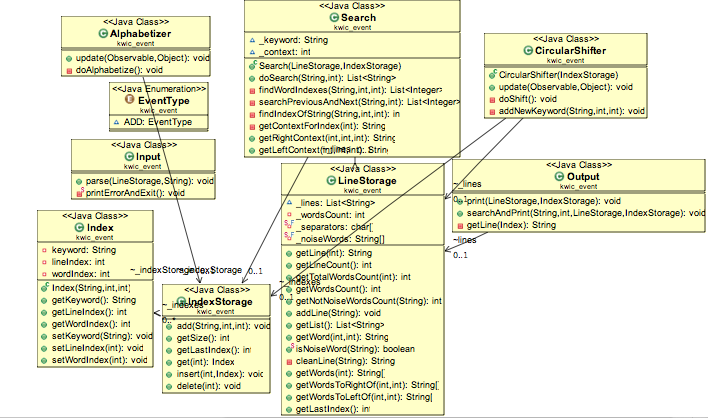
\includegraphics[width=13cm]{event}
	\label{fig:event}
\end{figure}

\section{Pipe-and-Filter}

Pipe and Filter architektura se skládá ze dvou základních typů objektů - rour a filtrů. Roura má na starosti řízení toků dat mezi jednotlivými filtry a sdílení paměti jiným způsobem než přímo přes rouru není možné. Každý filtr pak vykonává svou část práce ihned poté, co obdrží dostatečná data. V našem případě máme následující filtry: CircularShift, Alphabetizer, Search, NoiseFilter.  Oproti jiným implementacím přibyl NoiseFilter, který dělá filtraci noise words (slova, podle kterých nebudeme vyhledávat).

\begin{figure}[htbp]
	\caption{Pipe and Filer - class diagram}
		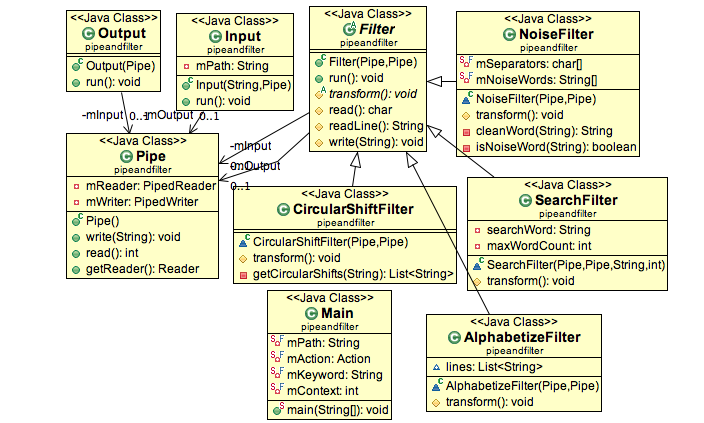
\includegraphics[width=13cm]{pipe}
	\label{fig:pipe}
\end{figure}

\section{Srovnání implementací}

\subsection{Zhodnocení kvality kódu, rozšiřitelnost, znovupoužitelnost}

Z hlediska kvality kódu je na tom poměrně dobře implementace používající Abstract Data Types vzhledem k tomu, že je možné jednoduše modul za jiný. Moduly na sobě mají jen jednoduché závislosti a jsou “decoupled”. Podobně dobře na tom z hlediska znovupoužitelnosti je i Pipe and filter, kde jsou jednotlivé moduly (filtry) zcela nezávislé a formát dat přenášený mezi nimi je jednotný - je tedy možné snadno vyměnit libovolný filtr za jiný nebo přidat další. Podobně je možné rozšičovat i Event based řešení pouhým zaregistrováním nového modulu jako Observer.

Co se změn v datové reprezentaci týče je na tom nejlépe Event based řešení, kde je k datům přistupováno abstraktně a jejich implementace může být snadno vyměněna. Naopak nejhůře je na tom  Shared memory, kde změna datového uložiště zasáhne prakticky všechny moduly a ty musí být změněny společně s datovým uložištěm.
Srovnání rychlosti

\subsection{Srovnání výkonu}

Pro otestování a srovnání rychlosti a paměťové náročnosti jsme si vybrali tři různé vstupy a na těch otestovali jednotlivé implementace. Jednalo se o dva medium.txt (5500 slov - článek o Dependency injection od Martina Fowlera) a big.txt (29949 slov - kniha Of Mice and Men od Johna Steinbecka).

\subsubsection{Test na malém souboru (hodnoty v ms)}

\begin{tabular}{|l||l|l|l|l|l|l|}
\hline
  {\bf }  & {\bf test1} & {\bf test2} & {\bf test3} & {\bf test4} & {\bf test5} & {\bf průměr}  \\
  \hline \hline
  Shared  & 5723& 5406 & 5475 & 5603 & 5556 & 5552  \\
  ADT  & 5401& 5460 & 5579 & 5349 & 5920 & 5541  \\
  Event  & 2577& 2655 & 2568 & 2654 & 2645 & 2619  \\
  Pipe and Filter  & 18069 & 15469 & 17429 & 15970 & 17811 & 16949  \\
\hline
\end{tabular}

\subsubsection{Test na velkém souboru (hodnoty v ms)}

\begin{tabular}{|l||l|l|l|l|l|l|}
\hline
  {\bf }  & {\bf test1} & {\bf test2} & {\bf test3} & {\bf test4} & {\bf test5} & {\bf průměr}  \\
  \hline \hline
  Shared  & 203232& 221096 & 204324 & 203101 & 202541 & 206858  \\
  ADT  & 256708& 228394 & 236890 & 221539 &224388 & 233583  \\
  Event  & 76227& 72489 & 75903 & 73991 & 73632 & 74448  \\
  Pipe and Filter  & 63429 & 60604 & 67150 & 65418 & 62943 & 63908  \\
\hline
\end{tabular}

Jako výkonostně výhodné řešení se v případě malého i velkého vstupu ukázala Event based implementace. V případě velkých vstupů si ale ještě lépe vedla implementace používající Pipe and Filter, která v případě menšího vstupu dopadla nejhůře. Poměrně špatné a navzájem podobné výsledky v obou případech podávaly implementace Shared memory a ADT.

\subsection{Srovnání paměťové náročnosti}

\subsubsection{Shared memory}

max. využití heapu - 13.37 MB

\begin{figure}[htbp]
	\caption{Shared memory - využití heapu}
		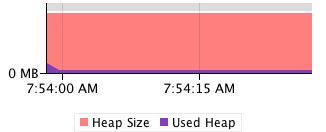
\includegraphics[width=7cm]{shared-memory}
	\label{fig:shared-memory}
\end{figure}

\subsubsection{ADT}

max. využití heapu - 15.09 MB

\begin{figure}[htbp]
	\caption{ADT - využití heapu}
		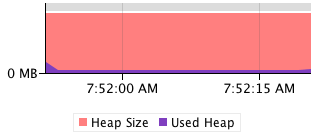
\includegraphics[width=7cm]{adt-memory}
	\label{fig:adt-memory}
\end{figure}

\subsubsection{Event based}

max. využití heapu - 16.69 MB

\begin{figure}[htbp]
	\caption{Event based - využití heapu}
		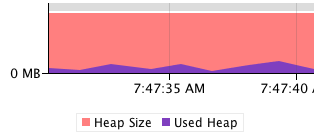
\includegraphics[width=7cm]{event-memory}
	\label{fig:event-memory}
\end{figure}

\subsubsection{Pipe and Filter}

max. využití heapu - 25.71 MB

\begin{figure}[htbp]
	\caption{Pipe and Filter - využití heapu}
		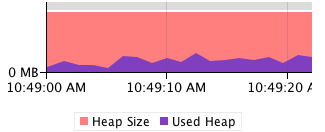
\includegraphics[width=7cm]{pipe-memory}
	\label{fig:pipe-memory}
\end{figure}

\subsubsection{Závěr}

Nejvíce paměťově náročné byla Pipe and Filter implementace, naopak nejlépe na tom bylo Shared Storage.

\end{document}  